
\subsubsection{Как стабилизируется положение РТ в транзисторе каскада на БТ?}
\begin{center}
	\begin{figure}[h!]
		\center{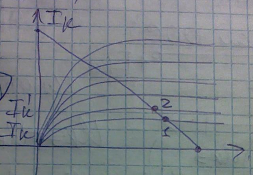
\includegraphics[scale=0.7]{22_VAX.png}}
		\caption{ВАХ}	
		\label{22_VAX}
	\end{figure}
\end{center}
При нагреве РТ смещается по нагрузочной прямой $\Rightarrow I_k$ увеличивается, $U_{ke}$ уменьшается$\Rightarrow$ транзистор приоткрывается$\Rightarrow$ при увеличении темпиратуры необходима темпиратурная стабилизация при помощи терморезистора, с помощью п/п диода
Принципиальная схема:
\begin{center}
	\begin{figure}[h!]
		\center{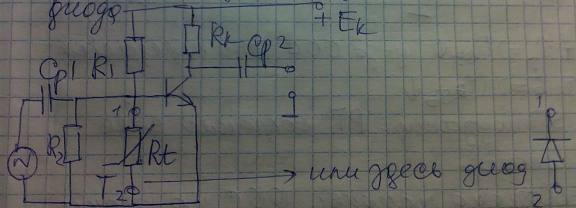
\includegraphics[scale=0.7]{22_Schem.png}}
		\caption{Cхема}	
		\label{22_Schem}
	\end{figure}
\end{center}
При росте T $R_T \downarrow\Rightarrow(R_2||R_t)\downarrow\Rightarrow U_{be}\downarrow\Rightarrow$ ЭП подзапирается и рабочая точка сохраняется.

Для Диода с увеличением T сопротивление в обратном включении $\downarrow$ засчет термогенерации носителей.

II способ: c помощью ООС
\begin{center}
	\begin{figure}[h!]
		\center{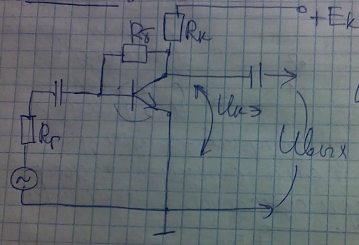
\includegraphics[scale=0.7]{22_Schem_OOS.png}}
		\caption{схема}	
		\label{22_Schem_OOS}
	\end{figure}
\end{center}
Из уравнений Кирхгофа $U_{ke}=U_{rb}+U_{be},U_{be}\downarrow=U_{re}\downarrow-U_{rb}$

$T\uparrow\Rightarrow U_{ke}\downarrow$ из-за ООС это передается на Б$\Rightarrow U_{be}\downarrow$

ЭП подхапирается, РТ сохраняет свое положение.

Можно использовать последовательную ООС по току
$$
U_2=U_{be}+U_{re},
U_2=const\Rightarrow
$$
$
I_k\uparrow\Rightarrow I_e\uparrow
$
\begin{center}
	\begin{figure}[h!]
		\center{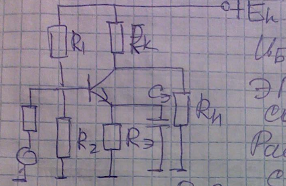
\includegraphics[scale=0.7]{22_Schem_OOS_Tok.png}}
		\caption{схема}	
		\label{22_Schem_OOS_Tok}
	\end{figure}
\end{center}

$U_{be}\downarrow$, но  сдругой стороны

$U_{be}\uparrow=U_2-U_{re}\uparrow$ЭП подзапирается, РТ сохраняет свое положение.

Рассмотрим коэффициенты усиления с ОС и без

$$
K_u=\frac{BR_H||R_k}{R_{вхтроэ}}$$
$$
\beta=\frac{U_{vixcoc}}{U_{vxcoc}}=\frac{I_kR_e}{I_kR_k}=\frac{R_e}{R_k}
$$

ОС отрицательная:
$$
K_{uos}=\frac{K_u}{1+\beta K_u}=\frac{K_u}{1+\frac{R_e}{R_k} K_u}\Rightarrow
$$
Чем больше $R_e$, тем стабильней схема

Т.О., при увеличении темпиратуры, $K_u\uparrow\Rightarrow\uparrow$ эквивалентное сопротивление входного контура$\Rightarrow I_b\downarrow\Rightarrow I_k$ растет меньше, чем без ОС
